% Hand-authored consolidated overview of the CVPR 2027 research package.
% Not produced by scripts/build_docs.py; compile with Tectonic from cvpr2027/:
%   .tools/tectonic docs/latex/research_overview.tex --outdir output/pdf --keep-logs
\PassOptionsToPackage{unicode}{hyperref}
\PassOptionsToPackage{hyphens}{url}
\PassOptionsToPackage{dvipsnames,svgnames,x11names}{xcolor}
\documentclass[11pt,a4paper]{article}
\usepackage{xcolor}
\usepackage[margin=24mm]{geometry}
\usepackage{amsmath,amssymb}
\usepackage{iftex}
\usepackage{lmodern}
\usepackage{textcomp}
\usepackage{parskip}
\usepackage{longtable,booktabs,array}
\usepackage{graphicx}
\usepackage{caption}
\usepackage{enumitem}
\usepackage{float}
\usepackage{needspace}
\usepackage{tikz}
\usetikzlibrary{arrows.meta,positioning,shapes.geometric,fit,calc}
\usepackage{hyperref}
% Shared style; used by generated, standalone LaTeX sources.
\usepackage{xcolor}
\usepackage{xurl}
\usepackage{fvextra}
\usepackage{etoolbox}
\usepackage{fancyhdr}
\usepackage{titlesec}
\definecolor{researchblue}{HTML}{173B58}
\AtBeginDocument{\hypersetup{linkcolor=researchblue,urlcolor=researchblue}}
\pagestyle{fancy}
\fancyhf{}
\fancyhead[L]{\small\sffamily SVG PATCH LAB}
\fancyhead[R]{\small\sffamily CVPR 2027 research package}
\fancyfoot[L]{\small Working documents; results and proposals distinguished}
\fancyfoot[R]{\thepage}
\setlength{\headheight}{15pt}
\setlength{\emergencystretch}{3em}
\titleformat{\section}{\Large\bfseries\color{researchblue}}{\thesection}{0.7em}{}
\titleformat{\subsection}{\large\bfseries\color{researchblue}}{\thesubsection}{0.7em}{}
\DefineVerbatimEnvironment{verbatim}{Verbatim}{breaklines=true,breakanywhere=true,fontsize=\small}
\AtBeginEnvironment{longtable}{\small\setlength{\tabcolsep}{4pt}}
\let\originaltableofcontents\tableofcontents
\renewcommand{\tableofcontents}{\originaltableofcontents\clearpage}

\captionsetup{font=small,labelfont=bf}
\setlist{nosep,leftmargin=1.4em}
\newcommand{\code}[1]{\path{#1}}
\newcommand{\degC}{\,\textdegree C}
\newcolumntype{L}[1]{>{\raggedright\arraybackslash}p{#1}}
\newcolumntype{R}[1]{>{\raggedleft\arraybackslash}p{#1}}
\hypersetup{pdftitle={Physics-consistent editing of engineering vector drawings: consolidated research overview},pdfauthor={SVG Patch Lab}}

\title{\color{researchblue}\LARGE Physics-consistent editing of engineering vector drawings\\[6pt]
\Large Consolidated research overview: problem, theory, architecture, experiments and plan}
\author{SVG Patch Lab \quad\textbullet\quad CVPR 2027 research package\\
\small branch \code{cvpr2027-research-package}; evidence at commit \code{cb3ab44}\\
\small plus \code{runs/colab-a100-20260916} and \code{runs/blackwell-20260917}}
\date{17 September 2026}

\begin{document}
\maketitle

\begin{center}
\small\itshape
Status: a proposal backed by limited diagnostic experiments. Not submission-ready; nothing has been submitted; author list and affiliations are pending. Every number below is copied from the packaged reports named at the end of each section.
\end{center}

\tableofcontents

% =====================================================================
\section{Problem statement}

\subsection{The question}

\textbf{Can an editable engineering drawing preserve the meaning of its numerical claims through natural-language presentation and physical edits, while remaining useful for drafting?}

An engineering drawing is both an image and a collection of claims. A curve marked 40\degC{} is a numerical assertion about every point on that curve. A stress legend asserts a quantity, a unit and a scale. Changing a load invalidates a previous solution even when its plot still looks plausible. Changing an ancestor SVG transform can invalidate geometry without changing the path string, and editing a text label can falsify a drawing while preserving every curve. The object that must be evaluated is therefore the \emph{final} drawing, together with the physical problem it depicts and the numerical evidence supporting it.

\subsection{Three separate questions}

A successful solver invocation answers none of the following automatically, and a low contour error answers only the second:
\begin{enumerate}
  \item Does the numerical solution adequately approximate the specified physical model?
  \item Does the displayed geometry agree with that solution within a stated numerical tolerance?
  \item Do the drawing's labels, units, legends and visibility agree with the intended claims?
\end{enumerate}

\begin{figure}[H]
  \centering
  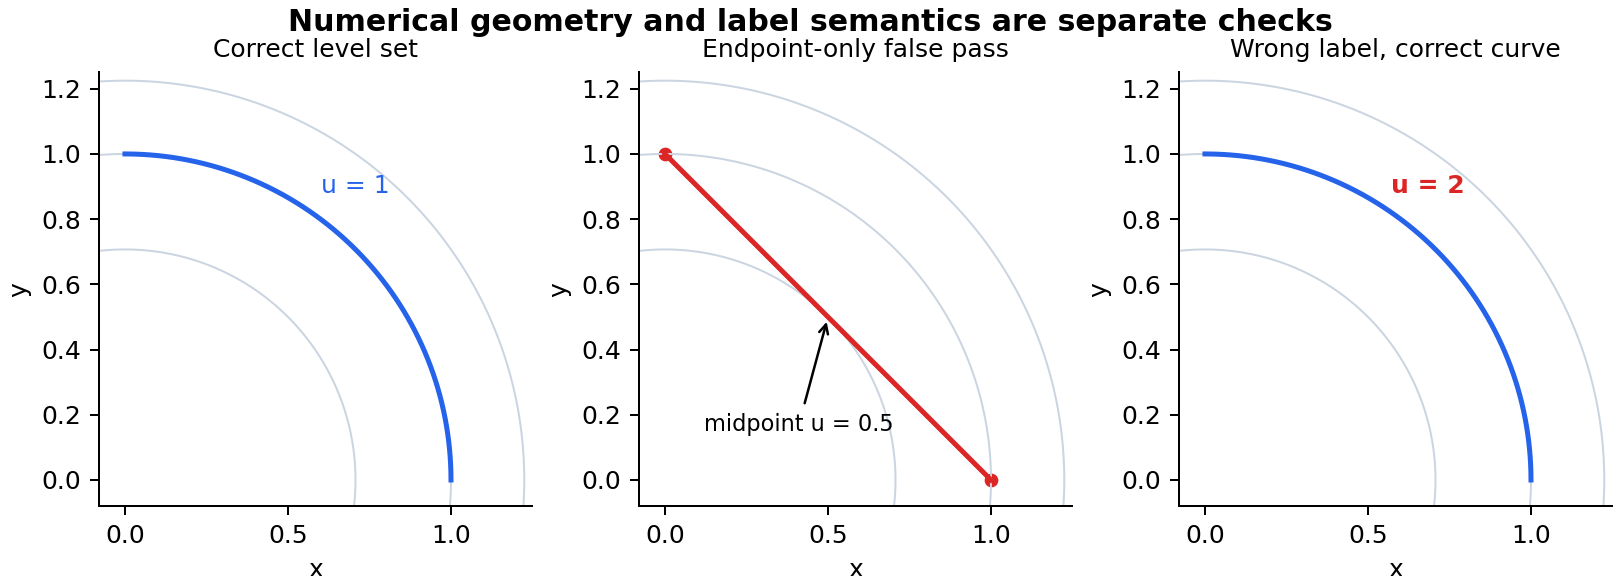
\includegraphics[width=\linewidth]{../../paper/figures/failure_modes.png}
  \caption[]{Numerical geometry and label semantics are separate checks. Left: a correct level set. Middle: endpoint-only checking accepts a chord whose midpoint value is $0.5$ instead of $1$. Right: a correct curve with a falsified label passes any purely geometric check.}
\end{figure}

\subsection{Why this is not ``LLM + FEM + SVG''}

Language models already formulate and execute simulations, generate scientific vector graphics and modify editable diagrams (Section~\ref{sec:prior}). The research problem is not whether a model can call a solver or output SVG. It is whether the final editable artifact remains consistent with the numerical solution it purports to depict, particularly after a sequence of natural-language edits, and whether protecting that consistency costs drafting usefulness.

\subsection{What a contribution would have to show}

The prospective submission must establish that a solver-linked representation improves \emph{useful} editing under a strong deterministic baseline and a prompting baseline, at comparable drafting quality. Without that evidence the work is a useful engineering audit rather than a demonstrated new computer-vision method. Three decision gates follow: (1) references and elementary integration pass before model comparisons; (2) the benchmark exposes a useful gap before large training; (3) a visual/graphics contribution survives the strongest controls before claiming CVPR readiness. If the gates fail, the claim is narrowed or the venue changed.

\emph{Sources:} \code{docs/source/research_proposal.md}, \code{paper/manuscript.md} \S1.

% =====================================================================
\section{Theory}

\subsection{Problem, solution record and drawing}

Let a physical problem be specified by domain geometry $\Omega$, governing equation $P$, boundary conditions $B$, material parameters $\theta$ and requested quantity $q$. A numerical solution record $R$ stores these inputs together with the solver and its version, the mesh or grid, units, convergence diagnostics and an identifier. Let $u_R$ be its scalar field and $D$ an SVG drawing associated with $R$.

A \emph{contour claim} consists of an SVG element identifier, a declared field level $c$, a quantity and unit, and a mapping from SVG coordinates to physical coordinates. The complete claim also includes the associated label and legend entry. Two edit classes follow:
\begin{itemize}
  \item A \emph{physical-input edit} produces a new problem and must invalidate the association with $R$ until a new solution is available. Changing a provenance identifier alone does not count; a real solve must occur.
  \item A \emph{presentation edit} must preserve the claims while changing only their visual arrangement or permitted style.
\end{itemize}
Requests that contradict the specification must be rejected or explicitly marked as illustrative. The representation must distinguish a computed field, a sampled geometric check, a schematic illustration and an unsupported claim. Content hashes record identity; they never prove that a solution is correct, and a reference solution must pass its own physical and numerical checks.

\subsection{Sampled geometric error}

For a sampled contour with physical points $x_i$ and arc-length weights $w_i$, the mean normalised geometric error in percentage points of the specified field range is
\begin{equation}
E_{\mathrm{mean}} = 100\,\frac{\sum_i w_i\,\lvert u_R(x_i)-c\rvert}{\operatorname{range}_R\,\sum_i w_i}.
\end{equation}
The maximum sampled error, required-level coverage, invalid-reference samples and unsupported rendering features are reported alongside it. The field range is fixed by the benchmark, not inferred per output. A \emph{strict pass} requires every required level, valid support for all checked samples, no flagged unsupported condition, and a maximum sampled error below the stated tolerance (0.5~pp of range for the historical re-audit; 0.5\degC{} for the Robin case).

Sampling intervals are bounded: a derivative-control-point bound for Bezier segments, a radius/angle bound and the affine operator norm for arcs. Samples include segment endpoints and never bridge disconnected subpaths; chord-length quadrature approximates arc-length weighting. Out-of-domain or masked samples are retained as invalid coverage rather than dropped. This is a numerical audit, not a mathematical certificate: finite sampling cannot prove correctness between samples, and reference interpolation has its own approximation error.

\subsection{Reference quality and error decomposition}

Three error sources are kept separate: \emph{reference error} (the numerical reference versus the continuum problem), \emph{output error} (the drawing versus the reference) and \emph{operational failure} (no output, truncated output, invalid SVG). A model is scored only against a reference that has passed analytic anchors, physical balance checks and mesh convergence. The engineering\_v4 design adds a \emph{reference floor}: every reference is computed at two resolutions and, where a second solver exists, cross-checked against it; the disagreement, measured as the $\varepsilon$ of one solver's isolines on the other's field, is the task floor, and a task whose floor exceeds 0.3~pp is rebuilt before use. Samples near a Dirichlet discontinuity are excluded from $\varepsilon$ only under a declared protocol, and full-domain results are always reported beside any exclusion.

The instantiated reference for the convective plate is steady conduction $\nabla^2 T = 0$ on $[0,2]\times[0,1]$ with $T=100\degC$ on the left edge and a Robin condition $\partial T/\partial n = -5T$ (ambient $0\degC$, $h/k = 5$) on the other three edges. In the P2 Galerkin weak form the Robin boundary integral $\int_{\Gamma_R} 5\,T\,v\,\mathrm{d}s$ is added to the stiffness form. Checks: an exact linear manufactured Robin anchor (error $2\times10^{-12}$), discrete heat balance between the assembled left reaction and the convective outflow ($\sim 10^{-13}$ relative), and five meshes from 576 to 147{,}456 triangles.

\subsection{Verifier outcomes and evaluation rules}

The verifier returns one of: \emph{accept within a stated scope}, \emph{report a limitation}, or \emph{request a repair or re-solve}. Unsupported features receive an explicit status rather than a silent pass, and a full-drawing certificate must not be reported until the visible-semantic scope is actually implemented and validated. Every attempted case is counted in denominators; API failures are operational outcomes, not evidence of PDE incapability. Physical cases are the unit of uncertainty: six edits of one case, or repeated seeds on one test set, are not independent samples.

\subsection{Hypotheses and falsification}

\Needspace{7\baselineskip}
\begin{longtable}{L{0.6cm} L{4.3cm} L{5.4cm} L{4.6cm}}
\toprule
ID & Hypothesis & Evidence required & Result that would weaken it \\
\midrule
H1 & Joint geometric and semantic checking reduces false acceptance after edits. & Fewer accepted wrong-field, wrong-unit and stale-solution outputs at comparable edit success. & Geometry-only or deterministic controls perform equally well. \\
H2 & A structured physical-edit path prevents reuse of stale fields. & Actual solver reruns and correct updated plots after load, material, boundary and geometry changes. & Provenance IDs change but plotted numbers remain stale. \\
H3 & Flexible protected editing is more useful than freezing the drawing. & Blinded drafting and instruction-fulfilment ratings improve without weakening numerical checks. & A simple plotting template matches quality and success. \\
H4 & Learning helps on context-dependent, visually grounded edits. & SFT improves over the same base model, executor and information on held-out cases and templates. & A rule parser or prompting closes the gap. \\
H5 & The method generalises beyond a single PDE or SVG template. & Independent geometry-family, instruction-template and sequential-edit holdouts. & Gains disappear when templates or layouts change. \\
\bottomrule
\caption[]{Hypotheses. The study must report negative results; a strong deterministic baseline is evidence about whether learned components are necessary, not a baseline to weaken.}
\end{longtable}

\emph{Sources:} \code{paper/manuscript.md} \S3--4; \code{docs/source/research_proposal.md}; \code{reports/ASTRA_FEM_FAILURE_RECHECK.md}; \code{reports/plan/engineering_v4_task_design.md} \S2.

% =====================================================================
\section{Architecture}

\subsection{Four records per artifact}

\Needspace{7\baselineskip}
\begin{longtable}{L{3.4cm} L{11.6cm}}
\toprule
Record & Contents \\
\midrule
1. Physical specification & Domain, dimensional assumptions, PDE, material law, loads, supports, boundary conditions, units, requested quantities. Unknown values remain explicit. \\
2. Numerical solution & Solver and version, discretisation, mesh, tolerances, fields, reactions/fluxes, convergence checks, provenance. \\
3. Drawing claims & SVG element IDs, physical-coordinate mapping, field quantity, contour level, associated text, unit and legend binding. \\
4. Edit record & Instruction, parsed operation, affected physical inputs or presentation properties, numerical invalidation, solver execution, verifier outcome. \\
\bottomrule
\end{longtable}

The engineering\_v4 encoding makes the claims machine-readable inside the SVG: \code{data-level} on every level set, \code{data-field} naming the field (\code{T}, \code{psi}, \code{phi}, \code{sigma_vm}), \code{data-quantity}/\code{data-value}/\code{data-unit} on every labelled scalar, and \code{data-status} $\in$ \{\code{solved}, \code{estimated}, \code{illustrative}\} on every field group, which turns disclosure into a self-report that can be checked against measurement. Every prompt fixes the \code{viewBox} and the affine map from physical to drawing coordinates.

\subsection{System components and data flow}

\begin{figure}[H]
\centering
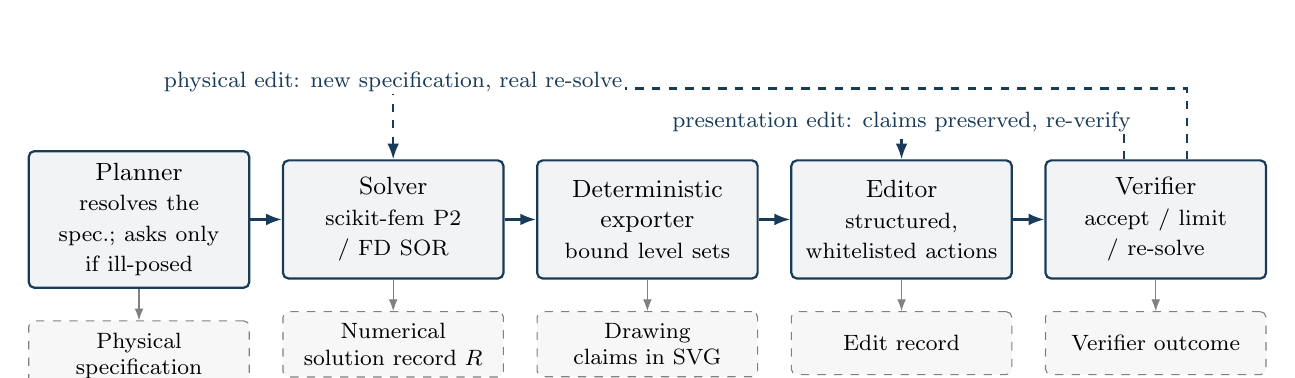
\begin{tikzpicture}[
  node distance=4mm and 4mm,
  box/.style={draw=researchblue,thick,rounded corners=2pt,fill=researchblue!6,align=center,minimum height=15mm,text width=25mm,inner sep=1.5mm,font=\small},
  rec/.style={draw=black!50,dashed,rounded corners=2pt,fill=black!3,align=center,minimum height=8mm,text width=25mm,inner sep=1.5mm,font=\footnotesize},
  arr/.style={-{Latex[length=2mm]},thick,researchblue},
  lbl/.style={font=\footnotesize,fill=white,inner sep=1pt}]
  \node[box] (plan) {Planner\\\footnotesize resolves the spec.; asks only if ill-posed};
  \node[box,right=of plan] (solve) {Solver\\\footnotesize scikit-fem P2 / FD SOR};
  \node[box,right=of solve] (exp) {Deterministic exporter\\\footnotesize bound level sets};
  \node[box,right=of exp] (edit) {Editor\\\footnotesize structured, whitelisted actions};
  \node[box,right=of edit] (ver) {Verifier\\\footnotesize accept / limit / re-solve};
  \draw[arr] (plan) -- (solve);
  \draw[arr] (solve) -- (exp);
  \draw[arr] (exp) -- (edit);
  \draw[arr] (edit) -- (ver);
  \node[rec,below=of plan] (r1) {Physical specification};
  \node[rec,below=of solve] (r2) {Numerical solution record $R$};
  \node[rec,below=of exp] (r3) {Drawing claims in SVG};
  \node[rec,below=of edit] (r4) {Edit record};
  \node[rec,below=of ver] (r5) {Verifier outcome};
  \foreach \a/\b in {plan/r1,solve/r2,exp/r3,edit/r4,ver/r5} \draw[-{Latex[length=1.5mm]},black!50] (\a) -- (\b);
  \draw[arr,dashed] ($(ver.north)+(-4mm,0)$) -- ++(0,4mm) -| (edit.north) node[lbl,pos=0.62,above] {presentation edit: claims preserved, re-verify};
  \draw[arr,dashed] ($(ver.north)+(4mm,0)$) -- ++(0,9mm) -| (solve.north) node[lbl,pos=0.55,above] {physical edit: new specification, real re-solve};
\end{tikzpicture}
\caption[]{Proposed system. Presentation edits preserve the physical solution but may change layout, line style and annotation position; physical edits create a new specification and trigger a new solve. Requests that contradict the specification are rejected or marked illustrative.}
\end{figure}

For the main study the verifier must inspect visible labels, units, legends and occlusion in addition to stored metadata; attaching a solution ID to an SVG is insufficient. Enforcement lives in code, not only in the model prompt.

\subsection{What is implemented today}

\begin{description}[style=nextline]
  \item[Geometric audit (\code{src/}, \code{scripts/field_fidelity.py}).] Parses SVG paths including arcs and reflected curve controls, composes ancestor and local transforms, samples by the bounds above, retains invalid samples, and refuses a strict pass on missing levels, malformed geometry or explicitly unsupported dynamic/rendering features. It always reports that a full drawing has not been verified.
  \item[Restricted editing executor.] Owns the generated SVG and exposes six actions: contour colour, bounded stroke width, moving a bound label within an annotation panel, routing a changed physical boundary for recomputation, rejecting a falsified numeric relabel, rejecting removal of a required contour. Geometry, level and transform mutations are refused; label text stays bound to its contour; a recomputation action returns a \emph{pending} solver request and never certifies the old field. The executor does not understand the instruction, so exact action fulfilment is scored separately from executor acceptance and geometry preservation.
  \item[Policy model.] Qwen2.5-Coder-1.5B-Instruct with attention-projection LoRA (rank 16, $\alpha=32$, dropout 0.05; 4{,}358{,}144 trainable parameters), receiving a compact DOM index and emitting one JSON action. It does not generate contour paths and does not see raster input.
  \item[Numerical references.] \code{scripts/robin_fem_reference.py} (scikit-fem P2, five meshes, analytic anchor, heat balance); \code{scripts/fem_bench_svg_extension.py} importing the unchanged MIT-licensed FEM-Bench axial-bar solver at commit \code{d370aef5}; FD red-black SOR with Robin support for rectilinear domains; a validated scikit-fem + Triangle plane-stress stack for general polygons with holes.
  \item[Deterministic controls.] A template rule parser (\code{scripts/eval_controlled_rule_baseline.py}), an explicit weak endpoint baseline, path-string hash protection and a rigid document freeze.
\end{description}

\subsection{Experiment and compute infrastructure}

\Needspace{7\baselineskip}
\begin{longtable}{L{5.4cm} L{9.6cm}}
\toprule
Component & Role \\
\midrule
\code{experiments/registry.json}, \code{scripts/experiments.py} & Registry of completed C01--C10 and planned P01--P08 with commands, dependencies and evidence paths. \texttt{run <ID>} reproduces CPU diagnostics into fresh timestamped directories; GPU and API jobs are never launched implicitly. \\
\code{notebooks/SVG_Colab_FEM_LoRA_20260916.ipynb}, \code{scripts/colab_run.py} & Single-cell A100 batch: downloads the pinned commit, installs recorded dependencies, runs nine stages with per-stage logs, resumes completed stages and checkpoints, exports an archive. \\
\code{scripts/remote_batch.py}, \code{remote_compute.py}, \code{bootstrap_remote.sh} & Same batch for a detached SSH host: prepare (hashed bundle) $\rightarrow$ connect $\rightarrow$ launch (\code{nohup}) $\rightarrow$ status $\rightarrow$ fetch; lock file, resume and source-hash checks; three runner tests. The supplied Serveo host \code{iit@sn4622130673} (RTX PRO 6000 Blackwell, 96~GB) ran the full batch on 17 September; the desktop session's 2~GB on the only GPU requires \texttt{launch -{}-gpu 0}. \\
\code{RUN_INDEX.json}, \code{SHA256SUMS.json}, \code{scripts/verify_package.py} & Evidence index and SHA-256 of 611 packaged files. Final adapters, trainer states, predictions and manifests are versioned; optimizer checkpoints and download archives stay local. No API credential is included. \\
\code{scripts/compare_reproduction.py} & Compares a fresh GPU batch with the saved run and references: exact on adapter bytes, predictions and loss history; tolerance on numerical references. \\
\bottomrule
\end{longtable}

\emph{Sources:} \code{docs/source/research_proposal.md} ``Proposed system''; \code{paper/manuscript.md} \S4; \code{reports/REMOTE_COMPUTE.md}; \code{cvpr2027/README.md}.

% =====================================================================
\section{Prior art and positioning}\label{sec:prior}

Two targeted audits were run (graphics side 12 September, FEM side 13 September). Their joint conclusion: \textbf{LLM + FEM, verified-code fine-tuning, multi-agent orchestration and multimodal input are not sufficient novelty claims.} The candidate extension is maintaining numerical and semantic correctness in the final editable drawing across edits. The search did not find a work implementing that whole contract, but the absence is not proof of novelty; the claim must be narrowed after reproducing the closest runnable systems.

\Needspace{7\baselineskip}
\begin{longtable}{L{3.2cm} L{5.8cm} L{5.8cm}}
\toprule
Work & What overlaps & Reuse or comparison \\
\midrule
MechAgents (EML 2024) & Agents formulate, execute and correct FEM elasticity programs; examples include plotting the wrong stress quantity. & Historical solver-agent baseline; notebooks pin older FEniCS/AutoGen versions. \\
MCP-SIM (npj AI 2026) & Language-driven simulation through tools and solver workflows. & Named simulation baseline; public tree lacks an imported \code{utils.py}, an entry point and a dependency manifest. \\
FEABench (2025) & End-to-end COMSOL problems with iterative tool feedback. & Executable call versus quantitatively correct solution; COMSOL is a dependency. \\
FEM-Bench (Dec 2025) & FEM function and test generation against reference and broken implementations. & Selected for code reuse (MIT). Its 33-task results are not comparable to SVG scores. \\
ALL-FEM (CMAME 2026) & Fine-tuned FEniCS code models; 1{,}000+ verified scripts; 3B--120B models. & Most direct precedent for the training component; training a solver agent alone is not new. \\
PDEAgent-Bench (2026) & 645 PDE instances, 11 families, three FEM tracks; accuracy beyond execution. & Calibrated-reference philosophy; keep its cases out of training. \\
OASiS (2026) & MCP access to several FEM solvers with verification and convergence studies. & Open-source orchestration baseline; scikit-fem backend. Documentation inspected, not reproduced. \\
VFEAgent (2026) & Image and text to structured FEA specification and code. & Multimodal drawing-to-FEA already exists; compare perception, specification and artifact separately. \\
ModSolAgent (TII 2026) & Abaqus scripting with retrieval, verification and distilled fine-tuning data. & Training precedent; Abaqus licensing must be checked. \\
Penrose (SIGGRAPH 2020) & Mathematical meaning separated from styling; constraint layout; SVG export. & Borrow semantics-versus-layout separation; contours must additionally be computed and bound. \\
SSVG-Bench / LOOP & Structural evaluation of scientific vector graphics. & Extend structural checks to PDE fields and edit sequences. \\
AutoFigure-Edit (ACL demo 2026), SciDiagramEdit (2026), SVGEditBench V2 (2025) & Editable scientific illustrations; instruction-driven revisions with skill evolution; general SVG editing. & Editing baselines and controls; add solver-derived claim checks. \\
FMforME (2026), SciForma (2026), Text2PDE (2024) & CAD-specification constraint checks; diffusion diagram generation; text-conditioned simulation. & Adjacent; not native SVG/PDE implementations. \\
\bottomrule
\caption[]{Closest prior work. Paper library: 20 source records, 15 downloaded PDFs, BibTeX and download provenance in \code{papers/}.}
\end{longtable}

\emph{Sources:} \code{reports/FEM_LITERATURE_AND_EXTENSION.md}; \code{reports/PRIOR_ART.md}; \code{papers/README.md}.

% =====================================================================
\section{Completed experiments C01--C10}

Each completed experiment has a runnable command and evidence under \code{runs/}. A planned experiment has no result; a working script is not evidence that a comparison was completed.

\Needspace{7\baselineskip}
\begin{longtable}{L{0.9cm} L{3.6cm} L{4.8cm} L{5.4cm}}
\toprule
ID & Scope & Evidence & Important limit \\
\midrule
C01 & Evaluator and edit-policy regressions & 30 passing tests & Tests cover implemented scope, not all SVG semantics. \\
C02 & Manufactured contour corruptions & 160 controls; audit accepts 20/120 corruptions & All remaining false accepts are wrong labels. \\
C03 & Historical v3 re-audit & Six attempts, three strict geometric passes & Corner and mask effects prevent blanket physics-failure claims. \\
C04 & Rule baseline & 60/60 test and 60/60 annulus & Shared templates make this pilot trivial. \\
C05 & A100 LoRA training & Three seeds, three epochs, 90 steps each; adapters saved & Same perfect scores as the rule baseline. \\
C06 & Astra API recheck & Four completed calls with raw responses and token usage & One sample per condition; not a failure-rate estimate. \\
C07 & Independent Robin FEM & Five meshes, analytic anchor, heat balance & Mesh differences are estimates, not certified bounds. \\
C08 & Direct FEM contour scoring & Maxima 0.111 and 0.374\degC & Finite sampling does not certify the entire drawing. \\
C09 & Historical capacitor path audit & 12 open field paths; no alleged closed loops & Source-specific geometry check, not electrostatic validation. \\
C10 & Upstream FEM-Bench SVG bridge & Two upstream tests and 24 FEM solves & A one-dimensional integration anchor only. \\
\bottomrule
\end{longtable}

\subsection{C01--C02: evaluator repair and manufactured corruption controls}

The audit found that the earlier evaluator sampled only segment endpoints, applied element-local transforms and dropped out-of-grid samples: in $u=x^2+y^2$ the chord \texttt{M 1 0 L 0 1} scored zero error although its midpoint is off by 0.5. The repaired evaluator is covered by 22 evaluator and 8 solver/edit-policy tests. Controls: 20 quarter-circle contour cases, each with two honest variants (unchanged, recoloured) and six corruptions (chord for arc, translated ancestor, changed level, hidden, removed, falsified label).

\Needspace{7\baselineskip}
\begin{longtable}{L{7.6cm} R{3.4cm} R{3.6cm}}
\toprule
Checker & Honest accepted ($n=40$) & Corrupt accepted ($n=120$) \\
\midrule
Explicit weak endpoint / local-coordinate baseline & 40/40 (100\%) & 80/120 (66.7\%) \\
Existing path-string hash protection & 40/40 (100\%) & 80/120 (66.7\%) \\
Repaired numerical geometry audit & 40/40 (100\%) & 20/120 (16.7\%) \\
Rigid document freeze except contour colour & 40/40 (100\%) & 0/120 (0\%) \\
\bottomrule
\caption[]{Manufactured corruption controls (\code{runs/contour-controls/}). The audit's 20 false accepts are all wrong-label cases: it does not verify text semantics. The freeze supports only the narrow colour edit tested. These are implementation controls with known construction, not prevalence estimates, and not evidence of superiority over the rigid baseline.}
\end{longtable}

\begin{figure}[H]
  \centering
  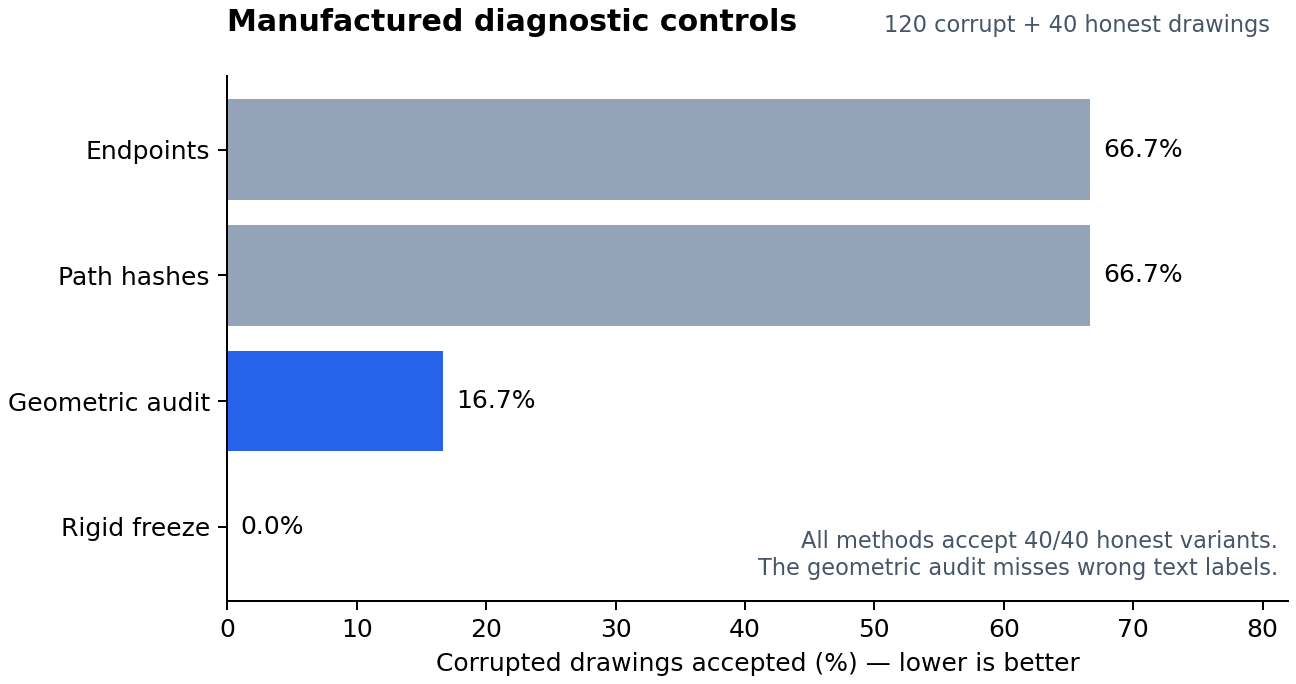
\includegraphics[width=0.9\linewidth]{../../paper/figures/corruption_controls.png}
  \caption[]{Corruption-control outcomes by checker and corruption type.}
\end{figure}

\subsection{C03: historical v3 re-audit}

Six pre-existing v3 generation attempts were rescored at a maximum sampled error of 0.5~pp of the specified range. Outputs and references were fixed before the repair; the threshold is exploratory, not preregistered.

\Needspace{7\baselineskip}
\begin{longtable}{L{3.6cm} R{1.7cm} R{1.7cm} R{2.2cm} L{5.4cm}}
\toprule
Attempt & Mean, pp & Max, pp & Invalid samples & Strict geometry pass \\
\midrule
L-shaped Laplace & 0.3537 & 80.0000 & 0 & No --- incompatible Dirichlet corners \\
Square torsion & 0.0701 & 0.3330 & 0 & Yes \\
Plate with square hole & 0.0693 & 0.2677 & 0 & Yes \\
Channel step streamlines & 0.0140 & 0.2459 & 0 & Yes \\
Square conductor in shell & 0.2167 & 0.3791 & 1{,}528 & No --- masked raster reference on boundary contours \\
Convective-edge plate & --- & --- & --- & No SVG returned; counted as attempted \\
\bottomrule
\caption[]{Historical re-audit (\code{runs/rescore-v3/}). Three strict passes out of six are not evidence of three incorrect physical solutions: the L-shape's largest discrepancies lie at incompatible corners and the shell's required interior contours have valid samples. A reference-domain protocol and mesh convergence are needed before assigning model error.}
\end{longtable}

\subsection{C04--C05: controlled-editing training pilot}

\textbf{Data.} 60 training physical cases $\times$ 6 edits $=360$ examples; validation, test and held-out annulus splits of 10 cases $\times$ 6 $=60$ each. Rectangular heat references are FD solves with analytic checks; annulus references are analytic. All variants of a case stay in one split (case-disjoint), but instruction templates are shared across splits, so this does not test language-template generalisation.

\textbf{Training.} FP16 frozen base, completion-only labels, micro-batch 4 $\times$ accumulation 3 $=$ effective 12, fixed three epochs $=90$ optimizer steps, seeds 17/29/41, no held-out-based selection. NVIDIA A100-SXM4-40GB, torch 2.11.0+cu128; about 95~s of training per seed; peak GPU memory 6.93~GB.

\Needspace{7\baselineskip}
\begin{longtable}{L{4.6cm} R{1.9cm} R{2.2cm} R{2.6cm} R{2.9cm}}
\toprule
Model / policy & Test strict & Annulus strict & Test fence-norm. & Annulus fence-norm. \\
\midrule
Base Qwen, each seed & 0/60 & 0/60 & 26/60 & 25/60 \\
Final LoRA, seed 17 & 60/60 & 60/60 & 60/60 & 60/60 \\
Final LoRA, seed 29 & 60/60 & 60/60 & 60/60 & 60/60 \\
Final LoRA, seed 41 & 60/60 & 60/60 & 60/60 & 60/60 \\
Deterministic template parser (C04) & 60/60 & 60/60 & 60/60 & 60/60 \\
\bottomrule
\caption[]{Pilot results: strict JSON exact action, and a sensitivity score removing one enclosing Markdown JSON fence. Train loss 0.0084/0.0082/0.0105; eval loss $\le 1.1\times10^{-4}$ by epoch 3. The base fails strict parsing mostly on fences but also makes action errors.}
\end{longtable}

\textbf{Interpretation.} Because the rule parser is perfect, the neural result is pipeline validation and does not show that learning is needed. Each split has only ten independent physical cases; repeated seeds do not add cases. Provenance: a first A100 run lost its weights before download; the recovery run repeated the configuration and is the only one counted (\code{reports/training_verified.json}).

\subsection{C06--C08: Astra API recheck against an independent FEM reference}

On 13 September four direct \code{gpt-6-astra} calls revisited the three suspected failure cases with the original prompts and wrapper, one sample per condition, \code{store=false}. All four finished with an SVG; total usage 1{,}312 input and 39{,}585 completion tokens ($\approx$\,\$1.99 at list price).

\Needspace{7\baselineskip}
\begin{longtable}{L{3.2cm} L{3.0cm} L{2.2cm} R{3.6cm} R{2.2cm}}
\toprule
Case & Effort / cap & Finish & Completion / reasoning tokens & Wall time \\
\midrule
Convective plate & medium / 16{,}000 & stop, SVG & 15{,}329 / 11{,}775 & 297.9 s \\
Convective plate & medium / 32{,}000 & stop, SVG & 17{,}697 / 14{,}660 & 334.3 s \\
Finite capacitor & low / 16{,}000 & stop, SVG & 3{,}120 / 512 & 48.8 s \\
L-bracket stress & low / 16{,}000 & stop, SVG & 3{,}439 / 512 & 63.2 s \\
\bottomrule
\end{longtable}

The independent reference (C07) is the Robin problem of Section~2.3. The last two meshes differ by at most 0.021\degC{} on the common grid and 0.008\degC{} at the sampled contour points; the old first-order FD reference differs from the fine FEM grid by up to 1.977\degC{} and is not ground truth. Direct evaluation in the FEM basis along the transformed SVG paths (C08), at a maximum physical step of 0.002, gives:

\Needspace{7\baselineskip}
\begin{longtable}{L{3.6cm} R{4.2cm} R{3.6cm} L{2.6cm}}
\toprule
New response & Arc-length-weighted mean & Maximum sampled error & Pass at 0.5\degC \\
\midrule
16{,}000-token cap & 0.00702\degC & 0.11074\degC & Yes \\
32{,}000-token cap & 0.01247\degC & 0.37385\degC & Yes \\
\bottomrule
\caption[]{The regular-grid audit gives slightly larger maxima (0.127 and 0.384\degC) because it adds interpolation error. Neither a benefit nor a disadvantage of the larger budget is established with one call per condition.}
\end{longtable}

\begin{figure}[H]
  \centering
  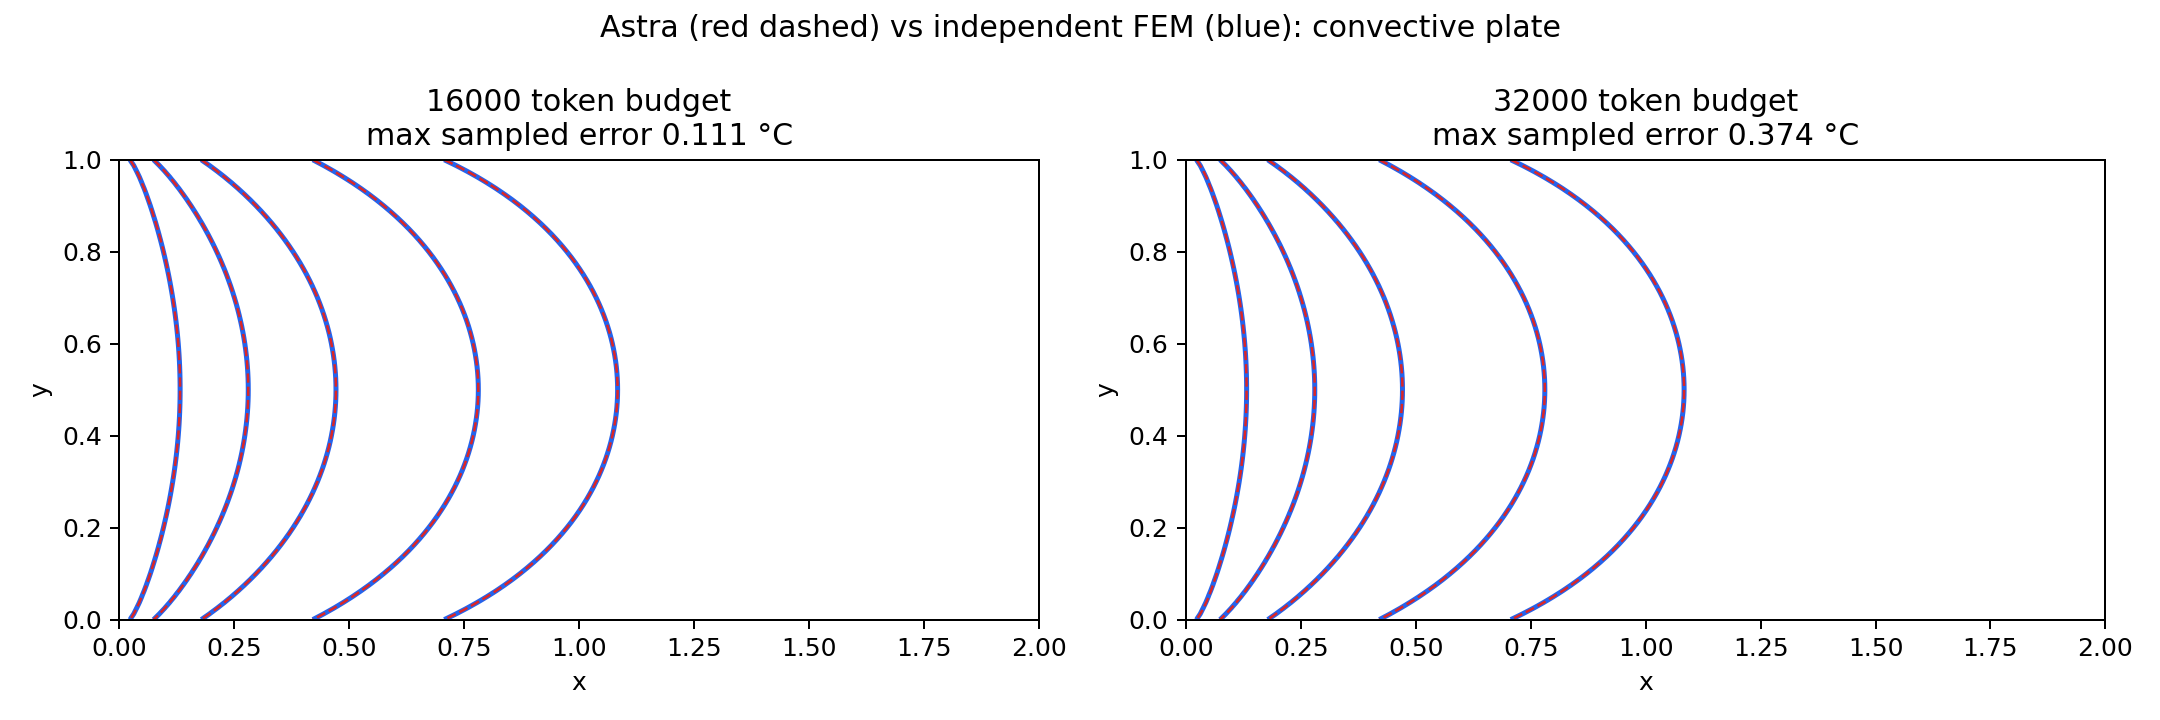
\includegraphics[width=\linewidth]{../../paper/figures/robin_fem_comparison.png}
  \caption[]{Astra contours (red dashed) over the independent FEM field (blue) for both token budgets.}
\end{figure}

\begin{figure}[H]
  \centering
  
\includegraphics[width=0.8\linewidth]{../../runs/robin-fem-reference/reference.png}
  \caption[]{The independent FEM reference for the convective plate (\code{runs/robin-fem-reference/}).}
\end{figure}

\subsection{C09: corrections to the earlier failure narrative}

\Needspace{7\baselineskip}
\begin{longtable}{L{2.6cm} L{3.6cm} L{8.8cm}}
\toprule
Case & Earlier claim & What the audit found \\
\midrule
Robin conduction & Beyond the model after one truncated call. & The historical call really did spend 16{,}000 reasoning tokens and return no SVG --- a real completion failure. Both new calls pass. One call cannot define a PDE-class limit. \\
Finite capacitor & Field lines form impossible closed loops. & 12 selected field paths, zero closed; every path joins the plates; the source says ``End contours schematic''. Maximum departure from field/equipotential perpendicularity $\approx 8.04^\circ$: approximate, not impossible. Fidelity is unverified, not disproven. \\
L-bracket & Wrong von Mises field. & Old and new outputs give $\approx 122$~MPa beam-theory nominal stress and illustrate a $\approx 220$~MPa hotspot with an assumed factor near 1.8, explicitly disclosed as not a solved FEM result. The prompt never specified fillet, support or contact; a sharp corner has no mesh-independent peak. \\
\bottomrule
\caption[]{The older overview and proposal claims are superseded; original files remain intact for provenance.}
\end{longtable}

\subsection{C10: reusing FEM-Bench --- a real solver in the edit loop}

\code{vendor/FEM-bench} is pinned to commit \code{d370aef5dbe023b0b86eb3548d24d11fd69328ee} with its MIT licence; the bridge imports the author's unchanged \code{FEM_1D_linear_elastic_CC0_H0_T0}. Both upstream reference tests pass. Twelve generated axial-bar cases plus twelve re-solves after a 50\% load increase give 24 actual FEM solves with displacements, reactions, provenance IDs and editable SVG plots for both states. Maximum analytic displacement error below $2\times10^{-18}$~m; maximum relative force imbalance below $4.2\times10^{-14}$. A stale old tip displacement would be 33.3\% low relative to the edited-load solution --- exactly the discrepancy a stale-field verifier must catch. This is not a reproduction of the FEM-Bench leaderboard, training on FEM-Bench, or a visual-reasoning result.

\emph{Sources:} \code{docs/source/experiment_protocol.md}; \code{reports/RESEARCH_STATUS.md}; \code{reports/TRAINING_RESULTS.md}; \code{reports/ASTRA_FEM_FAILURE_RECHECK.md}; \code{reports/FEM_LITERATURE_AND_EXTENSION.md}.

% =====================================================================
\section{New on 16--17 September 2026: two reproduction batches}

\subsection{Colab A100, 16 September}

One Colab A100 session executed the full packaged batch against commit \code{cb3ab448} in 15.6 minutes; all nine stages returned zero. The browser download \code{results-20260916T122720Z.tar.gz} (63{,}149{,}333 bytes, SHA-256 \code{e9be960f...}) matches the checksum printed in the notebook and is versioned in \code{runs/colab-a100-20260916/}. Stack: NVIDIA A100-SXM4-40GB; torch 2.11.0+cu128, transformers 4.51.3, peft 0.15.2, scikit-fem 12.0.2.

\Needspace{7\baselineskip}
\begin{longtable}{L{4.6cm} L{8.6cm} R{1.6cm}}
\toprule
Stage & Result & Wall time \\
\midrule
Regression tests & 30 passed & 20 s \\
Saved-adapter inference reload (\code{runs/a100}) & 18/18 exact actions, 0 unsafe edits --- this check had never been executed before & 60 s \\
LoRA training, seed 17 & 90 steps; train loss 0.008447; eval loss $6\times10^{-5}$; 60/60 test, 60/60 OOD & 220 s \\
LoRA training, seed 29 & 90 steps; train loss 0.008168; eval loss $6\times10^{-5}$; 60/60 test, 60/60 OOD & 240 s \\
LoRA training, seed 41 & 90 steps; train loss 0.010503; eval loss $1.1\times10^{-4}$; 60/60 test, 60/60 OOD & 220 s \\
New-adapter inference reload & 18/18 exact actions, 0 unsafe edits & 40 s \\
FEM-Bench axial bar & 2 upstream tests, 24 solves; analytic error $\le 5.3\times10^{-18}$~m; force balance $\le 4.1\times10^{-14}$ & 20 s \\
Robin conduction, $n=12\ldots192$ & heat balance $\le 3.4\times10^{-12}$; outflow$/k$ 260.816 $\rightarrow$ 259.918 with refinement & 40 s \\
Deterministic rule baseline & 60/60 test, 60/60 held-out family & 20 s \\
\bottomrule
\caption[]{Stage times are rounded up by the 20-second polling loop; training-only time per seed was 95.1, 97.1 and 93.8~s. Peak GPU memory 6.93~GB.}
\end{longtable}

\textbf{Agreement with the saved artifacts} (\code{scripts/compare_reproduction.py} $\rightarrow$ \code{reports/colab_reproduction.json}, \code{all_identical_or_within_tolerance} $=$ \texttt{true}):
\begin{itemize}
  \item The three new \code{adapter_model.safetensors} files are byte-identical to \code{runs/a100} (same SHA-256; 17{,}462{,}432 bytes; 4{,}358{,}144 parameters each).
  \item All 720 raw base and final predictions are identical; only the \code{batch_seconds} timing field differs. Split hashes, loss histories and manifests are identical apart from timing.
  \item FEM-Bench summary agrees to a maximum absolute gap of $6.3\times10^{-16}$~m; the Robin reference to $5.2\times10^{-10}$\degC{} across all meshes and derived comparisons.
\end{itemize}
Training on this stack is therefore deterministic across two separate A100 sessions, and the inference-reload check that was unexecuted when the earlier session disconnected has now passed twice. Identical outputs add no independent test cases; the pilot's interpretation is unchanged.

\emph{Sources:} \code{reports/COLAB_REPRODUCTION_20260916.md}; \code{reports/colab_training_verified.json}; \code{notebooks/SVG_Colab_FEM_LoRA_20260916_executed.ipynb}.

\subsection{Remote RTX PRO 6000 Blackwell, 17 September}

The same batch was run on the user-supplied Serveo SSH host (Ubuntu 24.04, 48 threads, 251~GB RAM, one NVIDIA RTX PRO 6000 Blackwell Workstation Edition with 97{,}887~MiB, driver 580.105.08) through \texttt{scripts/remote\_compute.py launch -{}-gpu 0}. The first attempt's GPU stages failed inside Triton: the default \code{torch==2.14.0} compiles a helper against \code{Python.h}, which the host's minimal Python lacks. Torch was pinned to \code{2.11.0} --- the version of both A100 runs --- and the batch resumed, skipping the four completed CPU stages. All nine stages passed by 15:53~UTC; artifacts are versioned in \code{runs/blackwell-20260917/}.

\Needspace{7\baselineskip}
\begin{longtable}{L{4.6cm} L{8.6cm} R{1.6cm}}
\toprule
Stage & Result & Wall time \\
\midrule
Regression tests; FEM-Bench bar; Robin $n=12\ldots192$; rule baseline & 30 passed; 24 solves with analytic error $\le 5.3\times10^{-18}$~m; heat balance $\le 3.4\times10^{-12}$ (finest solve 5.2~s on 48 threads); 60/60 and 60/60 & 8.1 s total \\
Saved-adapter inference reload & 18/18 exact actions, 0 unsafe edits & 8.4 s \\
LoRA training, seeds 17 / 29 / 41 & 90 steps each; train loss 0.008446 / 0.008165 / 0.010510; 60/60 test and 60/60 OOD for every seed; 35.2 / 34.4 / 35.8~s of training (A100: 95--97~s); peak 6.93~GB & 65.8 / 63.1 / 65.0 s \\
New-adapter inference reload & 18/18 exact actions, 0 unsafe edits & 8.2 s \\
\bottomrule
\end{longtable}

\textbf{Cross-architecture agreement} (\code{reports/blackwell_reproduction.json}: \code{functionally_equivalent} $=$ \texttt{true}, \code{all_identical_or_within_tolerance} $=$ \texttt{false}). Every one of the 360 final-model predictions is identical to the A100 run; base-model outputs differ in 1 of 120 generations per seed with unchanged scores; split hashes are identical; FEM references agree to $6.3\times10^{-16}$~m and $5.2\times10^{-10}$\degC. The adapter weights are not byte-identical: mean $|\Delta w|$ is $1.4$--$1.8\times10^{-4}$ and maximum $|\Delta w|$ about $6\times10^{-3}$ against a maximum $|w|$ of $3.1\times10^{-2}$, with per-tensor cosine similarity $\ge 0.972$ --- the size expected from non-associative floating-point accumulation over 90 optimizer steps on different CUDA kernels. Three hardware sessions (A100 twice, Blackwell once) therefore yield the same policies and predictions; the pilot's interpretation is unchanged.

\emph{Sources:} \code{reports/REMOTE_REPRODUCTION_20260917.md}; \code{reports/blackwell_training_verified.json}; \code{reports/REMOTE_COMPUTE.md}.

% =====================================================================
\section{Planned experiments P01--P08}

\Needspace{7\baselineskip}
\begin{longtable}{L{0.9cm} L{3.9cm} L{2.9cm} L{7.0cm}}
\toprule
ID & Purpose & Status & Acceptance criterion \\
\midrule
P01 & Numerical reference suite: heat, elasticity, electrostatics & Partial --- Robin anchor implemented & Reference metadata, physical-balance checks, convergence tables and error estimates for every case; unresolved cases stay in a diagnostic set. \\
P02 & Claim schema and complete verifier & Partial --- geometric only & Rejects specified corruptions and accepts honest counterfactuals; blind spots documented; no full-drawing certificate until visible semantics are validated. \\
P03 & Main case and edit collection & Designed & 240 cases across three families, split \emph{before} generating edits into 120/48/72; no case leakage; instructions require context beyond keyword routing. \\
P04 & Primary model and deterministic comparisons & Designed & Per-case results for every baseline with the complete attempted denominator. \\
P05 & Training study on a task that needs it & Designed & A reproducible, useful held-out gain, or a documented negative result. \\
P06 & Sequential physical and visual edits & Designed & Complete five-step traces with actual solver evidence, against a deterministic replotting baseline. \\
P07 & Ablations and robustness & Designed & Frozen development and evaluation sets; each ablation's changed capabilities explained. \\
P08 & Drafting and visible-correctness assessment & Designed & Three raters, agreement, exact rubric; sample chosen before viewing outcomes. \\
\bottomrule
\caption[]{Dependencies: P01/P02 precede main scoring; P03 precedes P04/P05; P06/P07/P08 support the final contribution claim.}
\end{longtable}

\subsection{P01 references and P02 verifier}

\emph{Heat:} steady 2-D conduction on rectangles and non-convex domains with Dirichlet, Neumann and Robin boundaries; Robin signs and corners validated with an analytic manufactured case and flux balance; at least three mesh levels. \emph{Elasticity:} finite plates with holes and rounded brackets with explicit geometry, $E$, $\nu$, plane-stress/strain choice, support model and distributed traction; displacement, force balance, free-surface traction and stress recovery checked; sharp-corner peaks unresolved unless the task asks for disclosure. A finite square plate differs from the infinite-plate Kirsch factor by 2\% ($K_t$ 3.086 vs 3.02--3.03), so every prompt states the full geometry and the reference is FEM on that geometry. \emph{Electrostatics:} 2-D versus 3-D, thickness, potentials and exterior boundary model stated; mesh and exterior domain both refined; conductor potential, symmetry, charge balance and field-line orthogonality checked.

P02 specifies solution IDs, quantity names, units, contour levels, coordinate maps, label anchors and legend mappings; defines invalidation for geometry, material, load and boundary changes; tests ancestor transforms, wrong scalar/tensor quantities, altered units, stale records, missing contours, hidden layers, clipping and label/legend mismatch; measures false acceptance on malicious and accidental corruptions; and includes honest edits that must be permitted.

\subsection{P03 collection and P04 baselines}

Each case includes presentation edits, label/legend edits, a physical-input edit, an under-specified request and an honest/misleading counterfactual pair; part of evaluation uses independently written requests with one provenance record each; geometry-family and instruction-template holdouts are stored separately. Test references, outputs and inspected failure corrections never enter training.

\Needspace{7\baselineskip}
\begin{longtable}{L{4.0cm} L{5.4cm} L{5.4cm}}
\toprule
Baseline & Input and freedom & What it isolates \\
\midrule
Direct Astra & Physical task and drawing; generates or edits SVG & Unaided final-artifact fidelity \\
Solver-informed unrestricted editor & Same numerical solution supplied; unrestricted SVG edits & Value of enforced protection beyond solver access \\
Published solver-agent workflow & Pinned runnable MechAgents / MCP-SIM / OASiS adaptation & End-to-end engineering workflow comparison \\
Protected geometry only & Numerical path protection; weaker annotation binding & Contribution of semantic checking \\
Joint geometry and semantics & Proposed representation and final verifier & Full proposed method \\
Deterministic solver plot / template & Solver-owned geometry and labels & Necessity and usefulness of learned drafting \\
Rigid freeze baseline & Minimal permitted style changes & Safety versus editing flexibility \\
\bottomrule
\caption[]{Identical specifications, references and requests where applicable; solver-access differences labelled; every attempted output preserved including invalid SVG and API failures; model alias, effort, token cap, endpoint, wall time and usage recorded.}
\end{longtable}

\subsection{P05--P08}

\begin{description}[style=nextline]
  \item[P05 training study.] Starts only after P03/P04 show a gap beyond the rule and deterministic controls. Base and SFT share executor and information; source, filtering and label generation recorded; completion-only supervision for structured actions; a small validation-driven search, then a three-seed final configuration with every tried configuration recorded. A multimodal claim requires a model that genuinely sees the image; a compact DOM index is not vision input.
  \item[P06 sequential edits.] Prespecified five-edit sequences: presentation change, physical parameter change, annotation rearrangement, geometry or boundary change, and a request that could reuse an old claim incorrectly; two-edit anchors for debugging. Every physical change invokes a real solver; caching only when the complete specification is unchanged. Per-step success, first failure, stale-solution acceptance, final visible correctness, cumulative latency and solver calls are tracked.
  \item[P07 ablations.] Remove one at a time: solver record, protected geometry, unit binding, legend binding, visibility checks, post-edit verification. Path-string freezing versus transformed-geometry checking; paraphrases, changed element IDs, nested transforms, alternate layouts and unseen geometry families. Corruptions are not retrofitted around the verifier's strengths; development and evaluation sets are frozen separately.
  \item[P08 human assessment.] Anonymised, randomised outputs from matched cases; raters judge instruction fulfilment, readability, numerical-label consistency and drafting suitability; three independent raters where feasible with agreement and rubric reported; sample fixed before viewing outcomes; numerical audits reported separately. No human study exists yet and none is fabricated.
\end{description}

\emph{Source:} \code{docs/source/experiment_protocol.md}.

% =====================================================================
\section{engineering\_v4 task design and the three-paper plan}

Plan SPL-PLAN-004 Rev~B (12 September) splits the programme into three papers and designs the benchmark tasks each needs. Its starting point was three earlier rounds --- 46 prompts, one model: drafting 46/46, closed-form physics 16/16, Dirichlet Laplace/Poisson exact on 7/7 ($\varepsilon \le 0.2$~pp), failures on Robin (no output), unbounded (undisclosed) and elasticity (decorative, disclosed). The 13 September recheck (Section~5.6) later softened the Robin and capacitor readings; the plan predates it.

\Needspace{7\baselineskip}
\begin{longtable}{L{2.6cm} L{4.8cm} L{1.6cm} L{3.4cm} L{2.4cm}}
\toprule
Paper & Thesis & Hyp. & Evidence needed & Status \\
\midrule
P1 --- Where the physics stops & A frontier LM drafts reliably and solves fixed-boundary 2-D potentials to solver accuracy, but fails on Robin, unbounded and tensor fields, and does not reliably disclose. & H1 (part), H2, H3, H5 & C1--C4 unaided, C6; $\ge 3$ models; $n=3$ samples; effort sweep on failing classes & 46-prompt study done; extended abstract now \\
P2 --- Solver in the loop & Solver output entering the SVG as protected geometry, with the model confined to constrained drafting patches, restores $\varepsilon<0.5$ on every class with no drafting loss. & H4 & WP2--WP4; B0/B1/B2 on C1--C5; seeded-corruption tests; C0 drafting control & $\varepsilon$ scorer and FD solver exist; after P1 feedback \\
P3 --- How does it solve Laplace? & The Dirichlet successes come from exploitable structure, not general numerical execution. & H1 (deep) & C1 knob sweeps, point-value probes, open-weight model with visible reasoning & 7 data points; standalone vs appendix TBD \\
\bottomrule
\end{longtable}

\textbf{Objections P1 will meet, and the design answers.} Single model? --- every class on $\ge 3$ models (astra, astra-pro, qwen3.8-27b, one more frontier model). Memorised textbook problems? --- anchor / textbook / procedural tiers, procedural tasks are seeded generators reported separately. $n=1$? --- $n=3$ per prompt $\times$ model $\times$ effort, mean and worst reported. Hidden code execution? --- tool-call fields logged, a point-value probe, replication on an open-weight model with visible reasoning. $\varepsilon$ only where it succeeded? --- $\varepsilon$, peak-location and topology checks defined for every class. No human rating? --- C0 rerun with a two-rater checklist on 20 drawings.

\Needspace{7\baselineskip}
\begin{longtable}{L{0.9cm} L{8.2cm} R{0.9cm} L{2.4cm} L{2.4cm}}
\toprule
Class & Content & Tasks & Reference & Feeds \\
\midrule
C0 & Drafting control (reuse v1). & 20 & --- & P1; P2 control \\
C1 & Dirichlet potentials on irregular domains: series and log anchors; L-shape and torsion; procedural rectilinear and simple polygons with holes; Poisson torsion; point-value probe. & 13 & series, log, FD, FEM & P1, P3 (H1) \\
C2 & Mixed and Robin boundaries: slab anchors; square plate with three convective edges at $\mathrm{Bi}\in\{0.1,1,10\}$; chip die; procedural mixed edges; token-budget $\times$ effort protocol. & 10 & closed form, FD & P1, P2 (H2) \\
C3 & Unbounded and open domains: line charges, cylinder flow, finite plates with \code{data-status}, charged square, Joukowski plate, parallel wires, procedural conductors; topology checks. & 8 & closed form, truncated FEM & P1, P2 \\
C4 & Elasticity with stress concentrators: Kirsch plate, edge holes, interacting holes, L-bracket with fillet $r\in\{2,8\}$~mm, U-notch, cantilever, procedural plate. & 10 & closed form + FEM & P1, P2 (H3) \\
C5 & Transient and nonlinear conduction: erfc slab, Heisler, square and L-shaped transients, $k(T)$ plate, radiating edge. & 6 & series, FD & P2 \\
C6 & Ill-posed and inconsistent specifications: inconsistent truss, all-Neumann with net flux, indeterminate beam, over-specified edge, unit trap, honest \code{data-status}. & 6 & none & P1 (H5) \\
\bottomrule
\caption[]{53 new tasks plus 20 reused from v1 and 3 from v2/v3. Rules: three tiers per class; fixed viewBox and physical map; two-resolution reference floor rebuilt if above 0.3~pp; two derivations where possible; metrics declared per task; one named difficulty knob; references rescorable from \code{runs/reference-v4/}.}
\end{longtable}

\textbf{Validated FEM stack (12 September).} L-shape Laplace FEM vs FD 0.007--0.010~pp away from the Dirichlet-jump corners; plate-with-hole free-surface radial stress $\le 0.002\,\sigma$ and net-section force ratio 0.9996--0.9998; long-strip $K_t$ 3.036 vs 3.02--3.03 tabulated; near-infinite plate hoop stress within 0.3\% of Kirsch; finite square plate $K_t$ 3.086 mesh-converged; under 1~s per reference.

\textbf{Build order.} (1) v4 manifest schema, \code{data-*} encoding, generalised \code{field_fidelity.py}, two-resolution floor; (2) C2 Robin budget sweep --- H2; (3) C6 ill-posed set --- H5; (4) C1 rectilinear procedural on FD --- H1; (5) scikit-fem + Triangle general polygons, C1.10--12; (6) plane stress, C4 --- H3; (7) truncated-domain FEM and topology, C3; (8) multi-model rerun of C0--C4, C6 at $n=3$ with effort sweeps $\rightarrow$ P1 full draft; (9) C5 and the WP3 protected level-set pipeline with B0/B1/B2 $\rightarrow$ P2 --- H4. First-reviewer packet: the overview PDF, the plan and five questions, to one FEM/heat-transfer reviewer, one language-model evaluator and one CAD/graphics reviewer, before step 5.

\emph{Source:} \code{reports/plan/engineering_v4_task_design.md} (repository root).

% =====================================================================
\section{Metrics, uncertainty, compute and stopping rules}

\begin{itemize}
  \item Report curve-field mean and maximum error normalised by an explicit field range, required-level coverage, unsupported samples, quantity/unit/legend errors, edit fulfilment, render validity, rejection/disclosure correctness, solver calls, latency and tokens; state whether errors come from direct FEM evaluation or grid interpolation.
  \item Physical cases are the resampling unit; paired case-level differences with confidence intervals when sample size permits; raw values published alongside.
  \item Reference error, output error and operational failure kept separate; full-domain metrics reported beside any prespecified singular-region analysis; a-posteriori exclusions are diagnostics only.
  \item A small feasibility batch first; tokens per case and wall time estimated before any large API study; a maximum job count and budget recorded in the run configuration; training jobs checkpoint and export automatically.
  \item Stop or redesign if references are unresolved, a task is under-specified, deterministic controls solve the main task, or the verifier is safe only by refusing useful edits. Validation selects models; sampling never continues until a preferred outcome appears.
\end{itemize}

% =====================================================================
\section{Risks and requirements before claiming a contribution}

\textbf{Principal risks:} reference error masquerading as model error; under-specified tasks (the bracket prompt never fixed fillet, support or contact); trivial templated edits solved by a rule parser; visual quality lost through over-restriction; overlap with prior systems. \textbf{Mitigations:} independent checks, explicit specifications, strong deterministic controls, blinded evaluation, a full baseline audit.

\textbf{Required before a CVPR claim:}
\begin{itemize}
  \item A real computer-vision/graphics contribution beyond a language-only action router.
  \item Public-code reproduction, or a clearly labelled reimplementation, of the closest runnable baseline with licence and environment preserved.
  \item Harder PDE geometry, Robin/elasticity cases, post-edit solver reruns, reference convergence, quantity/unit/legend binding, visibility and occlusion checks.
  \item Comparable drafting quality and edit success, including layout flexibility beyond a frozen template.
  \item Human-written or independently sourced instructions, held-out templates, multi-step edits, adversarial requests and honest counterfactuals.
  \item Prompt-only versus SFT with the same executor; unconstrained versus constrained editor; geometry-only versus semantic checks; plot/freeze/template controls.
  \item All attempted cases counted; per-task results; uncertainty by physical case; multiple seeds; compute and latency; verified citations; anonymisation; author review; final submission.
\end{itemize}

% =====================================================================
\section{Timeline to CVPR 2027}

\Needspace{7\baselineskip}
\begin{longtable}{L{4.2cm} L{10.8cm}}
\toprule
Working period & Required outcome \\
\midrule
13--20 September & Correct evaluator, calibrate references, define claim schema, freeze protocol. Evaluator and Robin/bar references done; claim schema partial. \\
21 September -- 4 October & Harder engineering/edit benchmark split by case and geometry family; baseline reproduction (P01--P03). \\
5--18 October & Main prompting and constrained-editor comparisons (P04); train only objectives with useful baseline gaps (P05). \\
19 October -- 1 November & Multiple seeds, ablations, sequential edits, mesh convergence, blinded drafting assessment (P06--P08). \\
2--9 November & Complete results, failure analysis, anonymised paper and reproducibility package. \\
10 November 2026 (AoE) & Paper registration deadline. \\
16 November 2026 (AoE) & Main paper deadline, after author review and approval. \\
23 November 2026 (AoE) & Supplementary material deadline. \\
\bottomrule
\caption[]{Work targets, not a promise of acceptance. Recheck the call and author guidelines (\url{https://cvpr.thecvf.com/Conferences/2027/Dates}); set up institutional OpenReview profiles early.}
\end{longtable}

% =====================================================================
\appendix
\section{Repository map}

\Needspace{7\baselineskip}
\begin{longtable}{L{4.6cm} L{10.4cm}}
\toprule
Path (under \code{cvpr2027/}) & Contents \\
\midrule
\code{docs/source/}, \code{docs/latex/}, \code{output/pdf/} & Proposal and protocol sources; generated and hand-authored LaTeX; review PDFs built with Tectonic. \\
\code{reports/} & Prior art, FEM survey, Astra/FEM recheck, training results, research status, Colab reproduction, remote compute; machine-readable \code{*_verified.json}, \code{colab_reproduction.json}, \code{package_verification.json}. \\
\code{paper/} & \code{manuscript.md} (working paper) and \code{figures/}. \\
\code{papers/} & 20 source records, 15 PDFs, \code{references.bib}, download manifest. \\
\code{src/}, \code{scripts/}, \code{tests/} & Evaluator and edit-policy modules; runnable experiments; 36 regression tests. \\
\code{data/}, \code{configs/} & Controlled-editing pilot splits; original prompts and historical SVG inputs. \\
\code{runs/} & \code{a100}, \code{colab-a100-20260916}, \code{blackwell-20260917}, \code{astra-api-recheck-20260913}, \code{robin-fem-reference}, \code{fem-bench-svg-anchor}, \code{contour-controls}, \code{rescore-v3}, \code{rule-baseline}, \code{astra-historical-audit}, \code{historical-v3}, \code{reference-v3}. \\
\code{vendor/FEM-bench/} & Unmodified MIT-licensed upstream files at commit \code{d370aef5}. \\
\code{experiments/}, \code{RUN_INDEX.json}, \code{SHA256SUMS.json} & Registry, evidence index, checksums. \\
\code{../reports/plan/} & \code{engineering_v4_task_design.md} (repository root). \\
\bottomrule
\end{longtable}

\section{How to reproduce}

\begin{verbatim}
python3 -m venv .venv && .venv/bin/python -m pip install -r requirements-local.txt
.venv/bin/python scripts/experiments.py list
.venv/bin/python scripts/experiments.py run C01   # 30 regression tests
.venv/bin/python scripts/experiments.py run C05   # verify saved training, recompute scores
.venv/bin/python scripts/experiments.py run C10   # FEM-Bench bridge, 24 solves
.venv/bin/python scripts/verify_package.py        # verify 611 packaged hashes
.venv/bin/python scripts/compare_reproduction.py --new runs/colab-a100-20260916 \
    --saved-training runs/a100 --saved-fem runs/fem-bench-svg-anchor/summary.json \
    --saved-robin runs/robin-fem-reference/summary.json --output reports/colab_reproduction.json
# GPU batch: run the single cell of notebooks/SVG_Colab_FEM_LoRA_20260916.ipynb on an A100
# Remote host: scripts/remote_compute.py prepare | connect | launch | status | fetch
# API repeat (billable, explicit): scripts/audit_astra_api.py --project . --output tmp/astra-new-run
\end{verbatim}

\section{Source documents consolidated here}

\begin{itemize}
  \item \code{docs/source/research_proposal.md} --- research proposal and alternative ideas.
  \item \code{docs/source/experiment_protocol.md} --- completed experiments, P01--P08, metrics, compute rules.
  \item \code{reports/PRIOR_ART.md}, \code{reports/FEM_LITERATURE_AND_EXTENSION.md} --- literature surveys and reuse decisions.
  \item \code{reports/ASTRA_FEM_FAILURE_RECHECK.md}, \code{reports/TRAINING_RESULTS.md}, \code{reports/RESEARCH_STATUS.md} --- completed results and failure audit.
  \item \code{reports/COLAB_REPRODUCTION_20260916.md} --- the 16 September reproduction batch.
  \item \code{reports/REMOTE_REPRODUCTION_20260917.md} --- the 17 September cross-architecture reproduction batch.
  \item \code{paper/manuscript.md} --- working paper.
  \item \code{reports/plan/engineering_v4_task_design.md} (repository root) --- three-paper split and task design.
\end{itemize}

\end{document}
